\chapter{Classes}

\section{What is a class?}

A class is a user-defined type. It specifies a blueprint for the creation of
objects. A class consists of a set of members:

\begin{itemize}
    \item Data members: variables that store the state of the object.
    \item Member functions (methods): functions that operate on the object.
\end{itemize}

The methods of a class can define the meaning of creation (constructor),
initialization, assignment, copy and cleanup (destructor), among other
operations, that determine the behavior of the objects of that class.

\section{Classes: \texttt{C++} general syntax}

In order to define a class in \texttt{C++}, we use the following syntax:\\

\begin{lstlisting}[language=C++]
class ClassName {
    public: // Accesible by all
        // functions
        // types
        // data (often best kept private!)

    private: // Accessible only by members of the class
        // functions
        // types
        // data
};
\end{lstlisting}

Notice that the members of a class can be public or private. Public members are
accessible from outside the class, while private members are only accessible
from within the class. A good practice is to keep the data members private and
provide public member functions to access and modify them. In that way, we can
control the access to the data and ensure that it is always in a valid state.\\

For example, we can define a class \texttt{Point} as follows:\\

\begin{lstlisting}[language=C++]
class Point {
    public:
        Point(int xx, int yy) : x(xx), y(yy) {} // Constructor
        int getX() { return x; }
        int getY() { return y; }
        void setX(int xx) { this->x = xx; }
        void setY(int yy) { this->y = yy; }
    private:
        int x;
        int y;
};
\end{lstlisting}

In this example, we define a class \texttt{Point} with two data members \texttt{x}
and \texttt{y} and four member functions: a constructor, two getter functions
\texttt{getX} and \texttt{getY}, and two setter functions \texttt{setX} and
\texttt{setY}.The members of a class can be accessed using the dot operator 
\texttt{.} for objects, and the arrow operator \texttt{->} for pointers to objects. 
Also, common operators such as \texttt{+}, \texttt{-}, \texttt{*}, \texttt{/}, 
among others, can be defined for a class.\\

Note that the public members of a class provide the class interface, while the private
members provide the class implementation. The class interface defines the
operations that can be performed on the objects of that class, while the class
implementation defines how those operations are performed.\\

Generally, we want to define the class interface, with all the public and private
member declarations, on a \texttt{.h} header file, while having the implementation of each 
function (including constructor and destructor) on a source \texttt{.cpp} file that 
includes this header. For example:

\begin{lstlisting}[language=C++]
// Point.h
#pragma once

class Point {
    public:
        Point(int xx, int yy); // Constructor
        int getX();
        int getY();
        void setX(int xx);
        void setY(int yy);
    private:
        int x;
        int y;
};
\end{lstlisting}

\begin{lstlisting}
// Point.cpp
#include "Point.h"

Point::Point(int xx, int yy) : x(xx), y(yy) {}
Point::getX() { return x; };
Point::getY() { return y; };
Point::setX(int xx) { x = xx };
Point::setY(int yy) { y = yy };
\end{lstlisting}

\section{Structs vs Classes}

In \texttt{C++}, the only difference between a \texttt{struct} and a \texttt{class}
is that the members of a \texttt{struct} are public by default, while the members
of a \texttt{class} are private by default. In general, we use \texttt{structs}
to define simple data structures, while we use \texttt{classes} to define more
complex data structures with associated operations.

\subsection{Structs in \texttt{C++}}

Structs are the simplest user-defined data structure that we have. As we said before, all its
members are public by default. This structure is inherited from the \texttt{C} language.
Its main syntax is:

\begin{lstlisting}[language=C++]
struct StructName {
    // data
    // Constructor
    // functions
};
\end{lstlisting}

For example, we can define a struct \texttt{Point} as follows:

\begin{lstlisting}[language=C++]
struct Point {
    int x;
    int y;
};
\end{lstlisting}

In general, we use structs to define simple data structures that group related
data together. Unlike classes, structs cannot define private members, so all
the date members of a struct are accessible from outside the struct.

\subsection{Public/private benefits}

The main benefit of using private members is that we can control the access to
the data and ensure that it is always in a valid state. For example, we can
define a class \texttt{Point} with private data members \texttt{x} and \texttt{y}
and provide public member functions to access and modify them. In that way, we
can ensure that the \texttt{x} and \texttt{y} coordinates of a point are always
non-negative.\\

In general, we use the public/private paradigm to:

\begin{itemize}
    \item Provide a clean interface to the users of the class.
    \item Hide the implementation details of the class.
    \item Allow the class to change its implementation without affecting its users.
    \item Easier to support code evolution.
    \item Mantain the class \textbf{invariants.}
\end{itemize}

\subsection{Invariants}

An invariant is a condition that must always be true for an object of a class.
It helps to ensure that the object is always in a valid state. For example, if we
define a class \texttt{Date} with data members \texttt{day}, \texttt{month} and
\texttt{year}, we can define, for example, the following invariants:

\begin{itemize}
    \item The day must be between 1 and 31.
    \item The month must be between 1 and 12.
    \item The year must be greater than 0.
\end{itemize}

We can enforce these invariants by defining the data members as private and
providing public member functions to access and modify them. In that way, we can
ensure that the \texttt{day}, \texttt{month} and \texttt{year} of a date are
always in a valid state.\\

In general, invariants help to ensure that the data that an object stores is always
correct and meaningful for its context. They help to prevent bugs and make the code 
easier to understand and maintain.\\

If we can't think of a good invariant for our data structure, we are probably dealing
with plain data, and if so, we may use a \texttt{struct} instead. But generally,
we should try to find good invariants for our user-defined types, so we can regularize
the behavior of our objects and prevent buggy code.

\section{\texttt{this} parameter}

When we call a member function, we do so on behalf of an specific object (an instance
of our class). Member functions access the object on which they were called through
an extra, implicit parameter named \texttt{this}. This parameter will be initialized
with the address of that object, so its data will be accesible from within the member
function.\\

For example, let us define a class that stores a date:\\

\begin{lstlisting}[language=C++]
class Date {
    public:
        Date(int dd, int mm, int yy) : d(dd), m(mm), y(yy) {}
        int day() { return d; }
        int month() { return m; }
        int year() { return y; }
    private:
        int d;
        int m;
        int y;
}
\end{lstlisting}

Then, when we call \texttt{object.month()} on a certain \texttt{object}, the compiler
automatically passes the address of that object to the method. Its if like the method 
were defined as:\\

\begin{lstlisting}[language=C++]
Date::month(Date *this) // Just a representation of what is happening
\end{lstlisting}

So, we have:

\begin{lstlisting}[language=C++]
Date my_birthday(26, 2, 2001);
int m = my_birthday.month()
// It is like we were writing Date::month(&my_birthday)
\end{lstlisting}

Note that inside the member functions, we are refering directly to the members of
the object on which the function was called, without using \texttt{this}.
Any direct use of a member of the class is assumed to be an implicit reference through
\texttt{this}. That is, when \texttt{month} uses \texttt{m}, it is as if we had
written \texttt{this -> m}.\\

It is then obvious that, when we define members methods of a class, it is forbidden to
use the keyword \texttt{this} for naming a parameter or a variable. Note that \texttt{this}
is a \texttt{const} pointer, meaning that we cannot change the address that it holds.

\section{\texttt{const} member functions}

When we define a member function of a class, we can specify that it is a \texttt{const}
member function by appending the \texttt{const} keyword to the function declaration.
A \texttt{const} member function is a member function that cannot modify the object
on which it was called.\\

For example, we can define a class \texttt{Date} with a \texttt{const} member function
\texttt{year} as follows:\\

\begin{lstlisting}[language=C++]
class Date {
    public:
        Date(int dd, int mm, int yy) : d(dd), m(mm), y(yy) {} // Constructor

        // ... Non-const member functions ...

        int year() const {
            ++y // (Imagine we do this by mistake)
            return y; 
        }
    private:
        int d;
        int m;
        int y;
}

Date my_birthday(26, 2, 2001);
int y = my_birthday.year(); // Will result in an error
\end{lstlisting}

In this example, we define a class \texttt{Date} with a \texttt{const} member function
\texttt{year} that tries to increment the year of the date. Since \texttt{year} is a
\texttt{const} member function, it cannot modify the object on which it was called.
Therefore, the statement \texttt{++y} will result in a compilation error.\\

In general, we use \texttt{const} member functions to ensure that the object on which
they were called is not modified. This helps to prevent bugs and make the code easier
to understand and maintain.\\

\section{Helper functions}

Helper functions are functions that are not members of a class, but that operate on
objects of that class. They are useful to define operations that are not part of the
class interface, but that are related to the class.\\

Usually, we want to keep the class interface clean and simple, and as minimal as
posible, so we define helper functions as non-member functions (outside the class) to
avoid cluttering the class interface, and when we need to define more complex operations.\\

For examplee, if we continue with the \texttt{Date} class, we can define a helper
function \texttt{next\_sunday()} that returns the next Sunday after a given date. We can
define this function as follows:\\

\begin{lstlisting}[language=C++]
class Date {
    // ... previous implementation ...
}

Date next_sunday(const Date &d) {
    // ... Implementation ...
    // returns a new Date object
}
\end{lstlisting}

Usually, we declare helper functions in the header file as the class, and define them
in the source file that includes the header. This way, we can keep the class interface
clean and simple, and provide the implementation details in the source file.

\section{Operator overloading}

In \texttt{C++}, we can define the behavior of operators for a class by overloading
them. Operator overloading allows us to define the meaning of operators such as
\texttt{+}, \texttt{-}, \texttt{*}, \texttt{/}, among others, for objects of a class.\\

When defining an operator for a class, we must define a member function or a non-member
function that specifies the behavior of that operator for objects of that class. The 
operator must have at leat one operand of the class for which it is defined.\\

Some advices for operator overloading are:

\begin{itemize}
    \item Define operators only when they make sense for the class.
    \item Define operators only with their conventional meaning.
    \item Don't overload operators like \texttt{*}, \texttt{\&\&}, \texttt{||}, \texttt{!}
\end{itemize}

\subsection{Operators as member functions}

When we define an operator as a member function, the object on which the operator
was called is the left operand of the operator, and the right operand is passed as
an argument to the member function.\\

For example, we can define the operator \texttt{+} for a class \texttt{Point} as a
member function as follows:\\

\begin{lstlisting}[language=C++]
class Point {
    public:
        // ... previous implementation ...

        Point operator+(const Point &p) {
            return Point(x + p.x, y + p.y);
        }

    private:
        // ... previous implementation ...
}
\end{lstlisting}

Note that the syntax for overloading an operator as a member function is to define
a member function with the name \texttt{operator} followed by the operator that we
want to overload. In this case, we define the operator \texttt{+} for the class
\texttt{Point} that adds two points.\\

We can also define operators between our class and other types. For example, when defining
the \texttt{[]} operator for a class, we can define it as a member function that takes
an integer as an argument. Let us see an implementation of this operator for a class
\texttt{Vector}:\\

\begin{lstlisting}[language=C++]
class Vector {
    public:
        // ... some implementation ...

        double &operator[](size_t i) const;

    private:
        std::vector<double> data;
}

double &Vector::operator[](size_t i) const { // Obs: returning a reference
    while (data.size() <= i) {
        data.push_back(0.);
    }
    return data[i];
}
\end{lstlisting}

In this example, we define the operator \texttt{[]} for the class \texttt{Vector} that
returns a reference to the element at the given index. If the index is out of bounds,
we push back zeros to the vector until the index is valid.\\

For operators as member functions, the left operand is always bounded to \texttt{this}.

\subsection{Operators as non-member functions}

When we define an operator as a non-member function, the object on which the operator
was called is passed as an argument to the function. This overloading is useful when
we want to define operators that are symmetric between two objects of the same class.\\

The syntax for overloading an operator as a non-member function is to define a non-member
function that takes two arguments of the class for which we want to overload the operator.\\

For example, we can define the operator \texttt{+} for a class \texttt{Point} as a
non-member function as follows:\\

\begin{lstlisting}[language=C++]
class Point {
        // ... some implementation ...
}

Point operator+(const Point &p1, const Point &p2) {
    return Point(p1.x + p2.x, p1.y + p2.y);
}
\end{lstlisting}

In this example, we define the operator \texttt{+} for the class \texttt{Point} as a
non-member function that adds two points. We have a problem here, because the operator 
\texttt{+} is not a member of the class \texttt{Point}, so it cannot access the private 
members of the class (in this case, \texttt{x} and \texttt{y}). To solve this, we can 
declare the operator \texttt{+} as a friend function of the class \texttt{Point}. 
It goes as follows:

\subsubsection{Friend functions}

When we define an operator as a non-member function, we can specify that the function
is a friend of the class. A friend function is a function that is not a member of the
class, but that has access to the private members of the class.\\

The syntax for defining a friend function is to declare the function as a friend of
the class in the class definition, and to define the function as a non-member function.\\

For example, we can define the operator \texttt{+} for a class \texttt{Point} as a
friend function as follows:\\

\begin{lstlisting}[language=C++]
class Point {
    public:
        // ... some implementation ...

        friend Point operator+(const Point &p1, const Point &p2);
}

Point operator+(const Point &p1, const Point &p2) {
    return Point(p1.x + p2.x, p1.y + p2.y);
}
\end{lstlisting}

In this example, we define the operator \texttt{+} for the class \texttt{Point} as a
friend function that adds two points. Now the operator \texttt{+} has access to the
private members of the class \texttt{Point}, so we can add two points without any
problem:\\

\begin{lstlisting}[language=C++]
    Point p1(1, 2);
    Point p2(3, 4);
    
    Point p3 = p1 + p2;
\end{lstlisting}

\subsection{Member vs non-member}

When we define an operator for a class, we can define it as a member function or as
a non-member function. The choice between the two depends on the context and the
semantics of the operator.\\

Here are some general guidelines for choosing between a member function and a non-member
function:

\begin{itemize}
    \item Must be member: \texttt{= [] () ->}
    \item Should be member:
        \begin{itemize}
            \item Compound assignments: \texttt{+= -= *= /=}, etc.
            \item Modify operator: \texttt{++ --}
        \end{itemize}
    \item Better non-member:
        \begin{itemize}
            \item Arithmetic operators: \texttt{+ - * /}
            \item Bitwise operators: \texttt{\& | \^}, etc.
            \item Comparison operators: \texttt{== != < >}, etc.
        \end{itemize}
    \item Better not overloaded: \texttt{* \&\& || !}
    \item Cannot be overloaded: \texttt{:: ?: .* .}
\end{itemize}

\subsection{Returning \texttt{this} object}

When we define an operator for a class, we can return the object on which the operator
was called by reference. This allows us to chain multiple operators together.\\

This is usually done when overloading the assignment operator \texttt{=} or the
compound assignment operators such as \texttt{+=}, \texttt{-=}, \texttt{*=}, \texttt{/=}.
For example, we can define the operator \texttt{+=} for a class \texttt{Point} as a
member function that returns the object on which the operator was called by reference:\\

\begin{lstlisting}[language=C++]
class Point {
    public:
        // ... some implementation ...

        Point &operator+=(const Point &p) {
            x += p.x;
            y += p.y;
            return *this;
        }
}
\end{lstlisting}

In this example, we define the operator \texttt{+=} for the class \texttt{Point} as a
member function that adds a point to another point and returns the object on which the
operator was called by reference. This allows us to chain multiple operators together:\\

\begin{lstlisting}[language=C++]
Point p1(1, 2);
Point p2(3, 4);
Point p3(5, 6);

p1 += p2 += p3;
\end{lstlisting}

\section{Functions overloading}

In \texttt{C++}, we can define multiple functions with the same name, as long as they
have different parameter lists. This is called function overloading. Function overloading
allows us to define multiple functions with the same name that perform different operations
depending on the arguments that they receive.\\

When we call an overloaded function, the compiler selects the function that best matches
the arguments that we pass to the function. The selection is based on the number and
types of the arguments that we pass to the function.\\

Note that the return type of a function is not considered when selecting an overloaded
function. Therefore, we cannot define two functions with the same name and parameter
list that differ only in their return type, as this would result in a compilation error.
To overload a function, we must define it with a different parameter list. Let us see
an example:\\

\begin{lstlisting}[language=C++]
int f(int x);
int f(int x, int y); // This is ok, because the number of parameters is different

int g(int x);
void g(int x); // This is not ok, because we are only changing the return type
\end{lstlisting}

Note also that the compiler will always choose the most specific function that matches
the arguments that we pass to the function. If there is no exact match, the compiler
will try to find the best match by performing implicit conversions on the arguments.
Look at the following example:\\

\begin{lstlisting}[language=C++]
void f(int x);
void f(double x);

f(1); // Calls f(int x)
f(1.0); // Calls f(double x)
\end{lstlisting}

In this example, we define two overloaded functions \texttt{f} that take an integer
and a double as arguments. When we call \texttt{f(1)}, the compiler selects the function
\texttt{f(int x} because the argument is an integer. When we call \texttt{f(1.0)}, the
compiler selects the function \texttt{f(double x} because the argument is a double.\\

It is important to notice that sometimes we can have ambiguity when calling an overloaded
function. This happens when the compiler cannot determine the best match for the arguments
that we pass to the function. In this case, the compiler will issue a compilation error.
For example, look at the following code:\\

\begin{lstlisting}[language=C++]
void f(int x, int y);
void f(double x, double y);

f(1, 2.6); // Ambiguity, in both cases we have to perform a conversion
\end{lstlisting}

We could also define default arguments for a function. This is useful when we want to
provide default values for some of the arguments of a function. For example, we can
define a function \texttt{f} with default arguments as follows:\\

\begin{lstlisting}[language=C++]
void f(int x, int y = 0, int z = 0) {
    // ... Implementation ...
}
\end{lstlisting}

In this example, we define a function \texttt{f} with three arguments \texttt{x}, \texttt{y}
and \texttt{z}, where \texttt{y} and \texttt{z} have default values of 0. This means that
we can call the function \texttt{f} with one, two or three arguments, and the missing
arguments will be replaced by their default values. For example, we can call the function
\texttt{f} as follows:\\

\begin{lstlisting}[language=C++]
f(1); // Calls f(1, 0, 0)
f(1, 2); // Calls f(1, 2, 0)
f(1, 2, 3); // Calls f(1, 2, 3)
\end{lstlisting}

\subsection{Overloading and \texttt{const} parameters}

When we are overloading a function, we have to be careful with the \texttt{const}
qualifier. If we define two functions with the same name and parameter list, but
one of them takes a \texttt{const} parameter, the compiler will consider them as
the same function. In other words, a parameter that has a top-level \texttt{const}
is indistinguishable from one that does not have it. For example:\\

\begin{lstlisting}[language=C++]
void f(int x);
void f(const int x); // This is not ok, because the compiler will consider them as the same function
\end{lstlisting}

Nonetheless, there is a distinction when the \texttt{const} qualifier is applied to
a pointer or a reference. In this case, the compiler will consider them as different
functions. For example:\\

\begin{lstlisting}[language=C++]
void f(int &x);
void f(const int &x); // This is ok
\end{lstlisting}

\subsection{Overloading a member function}

As with non-member functions, member functions can also be overloaded. The same function-matching
process is used for calls to member functions. The compiler will select the most specific
function that matches the arguments that we pass to the function.\\

In this case, we can overload member functions based on whether they are \texttt{const} or not.
For example, we can define a class \texttt{Point} with two member functions \texttt{getX}
that differ in their \texttt{const} qualifier as follows:\\

\begin{lstlisting}[language=C++]
class Point {
    public:
        int getX() { return x; }
        int getX() const { return x; }
    private:
        int x;
}
\end{lstlisting}

In this example, we define a class \texttt{Point} with two member functions \texttt{getX}
that differ in their \texttt{const} qualifier. The first function \texttt{getX} is a
non-const member function that returns the x-coordinate of the point, while the second
function \texttt{getX} is a \texttt{const} member function that returns the x-coordinate
of the point.\\

When we call the function \texttt{getX} on a \texttt{const} object of the class \texttt{Point},
the compiler will select the \texttt{const} member function \texttt{getX}. When we call the
function \texttt{getX} on a non-\texttt{const} object of the class \texttt{Point}, the compiler
will select the non-\texttt{const} member function \texttt{getX}.

\section{Constructors}

A constructor is a special member function that is called when an object of a class is
created. It is used to initialize the object and set its initial state. A constructor
has the same name as the class and no return type.\\

As other functiones in \texttt{C++}, constructors have a (possibly empty) parameter list, and
a (possibly empty) function body. A constructor may also be overloaded, meaning that we can
define multiple constructors for a class with different parameter lists. Unlike other functions,
constructors cannot be declared \texttt{const}.\\

\subsection{Default constructors}

Classes control default initialization by defining a special constructor known as the
default constructor. This constructor takes no arguments, and if it is not explicitly defined
by the programmer, the compiler will generate one.\\

The compiled-generated constructor is known as the synthesized default constructor. For most cases,
this constructor initializes each data member of the class as follows:

\begin{itemize}
    \item If there is an in-class initializer, it is used to initialize the data member.
    \item Otherwise, default-initialize the data member.
\end{itemize}

Note that the synthesized default constructor is generated only if no other constructors are
defined for the class. If we define any constructor for the class, the synthesized default
constructor will not be generated.\\

We cannot always rely on the synthesized default constructor, because it may not initialize
the data members of the class as we expect. For example, objects of built-in or compound types
(such as arrays and pointers) have undefined values when default-initialized. Therefore, we should
initialize those members inside the class or provide a user-defined default constructor.\\

Sometimes, the compiler is unable to generate a default constructor. This happens when the class
has a reference member, a const member, or a member of a class that has no default constructor.\\

Let us see an example of a class \texttt{Point} with a constructor:\\

\begin{lstlisting}[language=C++]
class Point {
    public:
        Point(int xx, int yy) {
            x = xx;
            y = yy;
        }
    private:
        int x;
        int y;
}
\end{lstlisting}

In this example, we define a class \texttt{Point} with a constructor that takes two integers
\texttt{xx} and \texttt{yy} as arguments and initializes the data members \texttt{x} and \texttt{y}
with those values. When we create an object of the class \texttt{Point}, the constructor is called
to initialize the object. If we do not define a constructor for the class, the compiler will generate
a default constructor that initializes the object with undefined values. In this case, because the
data members are \texttt{int}, they will be initialized with garbage values.

\subsection{Initialization lists}

In \texttt{C++}, we can initialize the data members of a class in the constructor using an
initialization list. An initialization list is a comma-separated list of data members of the
class followed by their initial values enclosed in parentheses.\\

The syntax for an initialization list is to define the data members of the class followed by
a colon and the initial values of the data members enclosed in parentheses. For example, we
can define a class \texttt{Point} with a constructor that initializes the data members \texttt{x}
and \texttt{y} using an initialization list as follows:\\

\begin{lstlisting}[language=C++]
class Point {
    public:
        Point(int xx, int yy) : x(xx), y(yy) {}
    private:
        int x;
        int y;
}
\end{lstlisting}

This is specially useful when we have const members, or references, or when we want to initialize
the members with a value that is not the default one. In that case, we need to use the initialization
list, because we cannot assign a value to a const member in the constructor body. For example:\\

\begin{lstlisting}[language=C++]
class ConstRef {
    public:
        ConstRef(int ii);
    private:
        const int i;
        int &ri;
}

// This is not ok
ConstRef::ConstRef(int ii) {
    i = ii; // Error, we cannot assign a value to a const member
    ri = ii; // Error, we cannot assign a value to a reference member
}

// This is ok
ConstRef::ConstRef(int ii) : i(ii), ri(i) {} // Ok
\end{lstlisting}

\subsection{Delegating constructors}

In \texttt{C++11}, we can define a constructor that delegates its initialization to another
constructor of the same class. This is known as a delegating constructor. A delegating
constructor is useful when we want to avoid code duplication by reusing the initialization
logic of another constructor.\\

The syntax for a delegating constructor is to call another constructor of the same class
using the constructor initializer syntax. For example, we can define a class \texttt{Point}
with two constructors that delegate their initialization to a third constructor as follows:\\

\begin{lstlisting}[language=C++]
class Point {
    public:
        Point() : Point(0, 0) {} // Delegating constructor
        Point(int xx, int yy) : x(xx), y(yy) {}
    private:
        int x;
        int y;
}
\end{lstlisting}

In this example, we define a class \texttt{Point} with two constructors: a default constructor
that delegates its initialization to another constructor that takes two integers as arguments,
and a constructor that takes two integers as arguments and initializes the data members \texttt{x}
and \texttt{y} with those values. When we create an object of the class \texttt{Point} using the
default constructor, the delegating constructor is called to initialize the object with the values
\texttt{0} and \texttt{0}.

\subsection{Copy, assignment and destruction}

When we define a class in \texttt{C++}, we must consider how the objects of that class are
copied, assigned and destroyed. By default, the compiler will generate a copy constructor, an
assignment operator and a destructor for the class.\\

The copy constructor is a special member function that is called when an object is copied. It
is used to create a new object that is a copy of an existing object. The assignment operator
is a special member function that is called when an object is assigned. It is used to assign
the value of one object to another object. The destructor is a special member function that
is called when an object is destroyed. It is used to clean up the resources that the object
has acquired.

\subsection{Defining a type member}

A type alias is a name that is a synonym for another type. We can define a type alias in one of 
two ways:

\begin{itemize}
    \item Using the \texttt{typedef} keyword:
    
    \begin{lstlisting}[language=C++]
    typedef double d; // d is a synonym for double
    typedef double *dp; // dp is a synonym for double*
    \end{lstlisting}

    \item Using the \texttt{using} keyword:
    
    \begin{lstlisting}[language=C++]
    using d = double; // d is a synonym for double
    using dp = double*; // dp is a synonym for double*
    \end{lstlisting}

\end{itemize}

We can define a type member inside a class to define a type alias that is specific to that class.
A type member is a type alias that is a member of a class. For example:\\

\begin{lstlisting}[language=C++]
class Screen {
    public:
        using pos = std::string::size_type;
    private:
        pos cursor = 0;
        pos height = 0, width = 0;
}
\end{lstlisting}

In this example, we define a class \texttt{Screen} with a type member \texttt{pos} that is a synonym
for \texttt{std::string::size\_type}. We can use the type member \texttt{pos} to define the type of
the data members \texttt{cursor}, \texttt{height} and \texttt{width} of the class \texttt{Screen}.
This way, we can ensure that the data members have the same type and are consistent with each other.


\section{\texttt{static} members}

Classes sometimes need members that are associated with the class itself, rather than with individual
objects of the class. For example, a bank account class might need a data member that holds the interest
rate for all accounts. In that case, we would want to associate the rate with the class, not with each 
individual account.\\

These members are called \texttt{static} members. When we declare a member of a class as \texttt{static},
it means that the member is shared by all objects of the class. This means that there is only one copy
of the \texttt{static} member, regardless of how many objects of the class are created.\\

Like any other member, static members can be either public or private. The type of a static data member
can also be \texttt{const}, reference, array, class type, and so on, and we can also define static methods.\\

Let us see an example of a class \texttt{Account} with a static data member \texttt{interestRate}:\\

\begin{lstlisting}[language=C++]
class Account {
    public:
        void calculate() { amount += amount * interestRate; }
        static double rate() { return interestRate; }
        
    private:
        std::string owner;
        double amount;
        static double interestRate;
}
\end{lstlisting}

Note that static member functions are not associated with any object. Therefore, they do not have a
\texttt{this} pointer. This means that they cannot access non-static members of the class. So, for 
this same reason, declaring a static member function as \texttt{const} is meaningless.\\

Even though static members are not part of the objects of its class, we can use an object, reference or pointer
of the class to access the static members. For example:\\

\begin{lstlisting}[language=C++]
Account myAccount;
double r = myAccount.rate(); // Ok
\end{lstlisting}

Because static data members are not part of individual objects of the class type, they are not defined
when we create objects of the class. As a result, they are not initialized by the class cosntructors.
We may not initialize a static data member inside the class, instead we must define and initialize each
static data member outside the class body, and like any other object, a static data member may be 
defined only once.\\

Like global objects, static data members are defined outside any function. Once they are defined, they
continue to exist until the program completes.

\section{Copy constructors and destructors}

Each class defines a new type and the operations that objects of that type can perform.
When we copy, assign or destroy objects of a class, this class controls how these operations
are performed. Collectively, these operations are known as the \textbf{copy-control} operations.\\

IF a class does not define all the copy-control operations, the compiler will define them for us.
As a result, many classes can ignore the copy-control operations. However, there are some classes
that must define these operations, as relying on the compiler-generated versions would lead to
incorrect behavior. Usually, the hardest part of implementing copy-control operations is 
recognizing when they are needed.

\subsection{Copy-assigment operator}

Just as a class controls how the objects are initialized, it also controls how they are assigned.
The copy-assignment operator is a special member function that is called when an object 
is assigned to another object. It is represented by the \texttt{=} operator.\\

Just as it does for the copy constructor, the compiler defines a synthesized copy-assignment
operator for classes that do not define their own. The synthesized copy-assignment operator
assigns each non-static member of the right-hand object to the corresponding member of the
left-hand object. If some members cannot be copy-assigned, the synthesized copy-assignment operator
will not be defined. Array members are assigned by assigning each element of the array.\\

The synthesized copy-assignment operator returns a reference to its left-hand object. This allows
assignments to be chained.\\

We can define our own copy-assignment operator for a class. The copy-assignment operator is a member
function that takes a single parameter of the class type. Let us see an example of a class 
\texttt{SalesData} with a copy-assignment operator:\\

\begin{lstlisting}[language=C++]
class SalesData {
    public:
        SalesData &operator=(const SalesData &);
    private:
        std::string bookNo;
        unsigned unitsSold = 0;
        double revenue = 0.0;
}

SalesData &SalesData::operator=(const SalesData &rhs) {
    bookNo = rhs.bookNo;
    unitsSold = rhs.unitsSold;
    revenue = rhs.revenue;
    return *this;
}
\end{lstlisting}

In this example, we could also want that when we copy an object of the class \texttt{SalesData},
everything is copied except the \texttt{bookNo}. In that case, we could define the copy-assignment
operator as follows:\\

\begin{lstlisting}[language=C++]
SalesData &SalesData::operator=(const SalesData &rhs) {
    if (this != &rhs) {
        unitsSold = rhs.unitsSold;
        revenue = rhs.revenue;
    }
    return *this;
}
\end{lstlisting}

\subsection{Copy initialization}

When we use direct initialization, i.e., when we use the \texttt{Object(values)} syntax, 
we are asking the compiler to use ordinary function matching to select the constructor 
that best matches the arguments we provide.\\

When we use copy initialization, i.e., when we use the \texttt{Object = values} syntax,
we are asking the compiler to copy the right-hand object into the left-hand object, 
converting that operand if necessary.\\

Copy initialization ordinarily uses the \textbf{copy constructor}. This happens not only 
when we define variables using an \texttt{=}, but also when we:

\begin{itemize}
    \item Pass an object as an argument to a parameter of non-reference type
    \item Return an object from a function that has a non-reference return type
    \item Brace initialize the elements in an array or the members of an aggregate
    class
\end{itemize}

Also, some class types use copy initialization for the objects they allocate. The library
containers copy initialize their elements when we initialize the container, or when we 
call an insert or push member.

\subsection{Copy constructor}

A constructor is called the \textbf{copy constructor} if its first parameter is a
reference to the class type and any additional parameters have default values.
For example:

\begin{lstlisting}[language=C++]
class Foo {
    public:
        Foo(); // Default constructor
        Foo(const Foo &); // Copy constructor
}
\end{lstlisting}

Not that the first parameter must be a reference type: almost always a \textbf{reference to const},
although we can define the copy constructor to take a reference to non-const.\\

When we do not define a copy constructor, the compiler tries to synthesize one for us.
Unlike the synthesized default constructor, the synthesized copy constructor is defined
even if we define other constructors.\\

Note that if all members of a class can be copied (i.e., they have copy constructors),
the synthesized copy constructor member-wise copies each member of its argument into the
corresponding member of the object being created. If some members cannot be copied, the
synthesized copy constructor is unavailable (implicitly deleted).\\

We can define our own copy constructor for a class. For example, we can define a class
\texttt{SalesData} with a copy constructor as follows:\\

\begin{lstlisting}[language=C++]
class SalesData {
    public:
        SalesData(const SalesData &);
    private:
        std::string bookNo;
        unsigned unitsSold = 0;
        double revenue = 0.0;
}

SalesData::SalesData(const SalesData &orig) : 
    bookNo(orig.bookNo), 
    unitsSold(orig.unitsSold), 
    revenue(orig.revenue) 
{}
\end{lstlisting}

An important remark: container elements are copies. When we use an object to initialize
a container, or insert an object into a container, a copy of that object is placed in the
container, not the object itself. Just as when we pass an object to a non-reference
parameter, there is no relationship between the element in the container and the object
from which that value originated. Subsequent changes to the element in the container
have no effect on the original object, and vice versa.

\subsection{Destructors}

The destructore does whatever operations the class designer wishes to have executed
after the last use of an object. Typically, the destructor frees the resources that
the object acquired during its lifetime.\\

The destructor operates inversely to the constructors. And just as a constructor has 
an initialization part and a function body, a destructor has a function body and a
destruction part.\\

In a destructor, there is nothing akin to the constructor initializer list to control
how members are destroyed. The destruction part is implicit.\\

Let us compare the constructor and destructor of a class:

\begin{itemize}
    \item \textbf{Constructors} initialize the non-static data members of an object 
    and may do other work.
    \begin{itemize}
        \item Members are initialized before the function body is executed.
        \item Members are initialized in the same order as ther appear in the class.
    \end{itemize}

    \item \textbf{Destructors} do whatever work is needed to free the resources used by
    an object and destroy the non-static data members of the object.
    \begin{itemize}
        \item The function body is executed first and then the members are destroyed.
        \item Members are destroyed in the reverse order from which they were initialized.
    \end{itemize}
\end{itemize}

What happens when a member is destroyed depends on the type of the member. Members of 
class type are destroyed by running the member's own destructor. The built-in types
do not have destructors, so nothing is done t destroy members of built-in type.\\

The destructor is a member function with the name of the class prefixed by a tilde (\texttt{\~}).
It has no return value and takes no parameters. Because it takes no parameters, a destructor
cannot be overloaded, so there is always only one destructor for a class. The syntax is as
follows:\\

\begin{lstlisting}[language=C++]
class Foo {
    public:
        ~Foo(); // Destructor
        // ...
}
\end{lstlisting}

The destructor is called automatically whenever an object of its type is destroyed. This
happens on the following situations:

\begin{itemize}
    \item Variables are destroyed when they go out of scope.
    \item Members of an object are destroyed when the object of which they are a part
    is destroyed.
    \item Elements in a container, whether a library container or an array, are destroyed
    when the container is destroyed.
    \item Dynamically allocated objects are destroyed when the delete operator is applied
    to a pointer to the object.
    \item Temporary objects are destroyed at the end of the full expression in which they
    were created.
\end{itemize}

The compiler synthesizes a destructor for a class if the class does not define one. 
As with the copy constructor and copy-assignment operator, for some
classes, the default destructor cannot be synthesized.\\

A synthesized destructor works by calling the destructors of the members in reverse order
of their declaration. These members are destroyed as part of the implicit destruction
phase tha follows the destructor body.

\section{Copy control}

There are three basic operations to control copies of class objects:

\begin{itemize}
    \item Copy constructor
    \item Copy-assignment operator
    \item Destructor
\end{itemize}

There is no requirement that we define all these operations, but ordinarily we should
think of these operations as a unit. If we define one of these operations, we should
define all three. This is known as the \textbf{Rule of three}.\\

Although many classes need to define all (or none of) the copy-control members, some classes
have work that need to be done to copy or assign objects but has no need for the destructor.\\

For example, consider a class that gives each object its own, unique serial number:
\begin{itemize}
    \item Such a class would need a copy constructor to generate a new, distinct serial
    number for the object being created.
    \item That constructor would copy all the other data members from the given object.
    \item This class would also need its own copy-assignment operator to avoid assigning
    to the serial number of the left-hand object.
    \item This class would have no need for a destructor.
\end{itemize}

This example gives rise to a second rule of thumb: if a class needs a copy constructor,
it almost surely needs a copy-assignment operator as well, and vice versa. Nevertheless,
needing either the copy constructor or the copy-assignment operator does not (necessarily)
indicate the need for a destructor.\\

Another rule of thumb to use when you decide whether a class needs to define its own versions 
of the copy-control members is to decide first whether the class needs a destructor. Often,
the need for a destructor is more obvious that the need for the copy constructor or
assigment operator. If the class \textbf{needs a destructor}, it almost surely
\textbf{needs a copy constructor} and a \textbf{copy-assignment} operator as well.

\subsection{Using default and delete}

In \texttt{C++11}, we can use the \texttt{default} and \texttt{delete} keywords to control
the synthesized copy-control members. The \texttt{default} keyword tells the compiler to
generate the default version of a member function. This can prevent custom implementation
and improves code readability. For example:\\

\begin{lstlisting}[language=C++]
class SalesData {
    public: 
    // copy control; use defaults
    SalesData() = default;
    SalesData(const SalesData&) = default;

    SalesData& operator=(const SalesData&);
    ~SalesData() = default;

    // other members
};

SalesData& SalesData::operator=(const SalesData&) = default;
\end{lstlisting}

For some classes, there really is no sensible meaning for create a copy, so copies or
assigments must be denied. For example, the \texttt{iostream} classes prevent copying 
to avoid multiple objects to write or read from the same IO buffer.\\

To prevent (deny) the copyong behavior, in \texttt{C++} we use \textbf{deleted functions}.
To define a function as deleted, we use the same syntax as default, but using \texttt{delete}
afte the $=$ operator. This prevents the compiler to automatically synthesize the functions
declared as deleted. For example:\\

\begin{lstlisting}[language=C++]
struct NoCopy{
    NoCopy() = default;

    // disallow copy
    NoCopy(const NoCopy&) = delete;
    // disallow assignment
    NoCopy &operator=(const NoCopy&) = delete;

    ~NoCopy() = default;

    // other members
}
\end{lstlisting}

\subsection{Resource management}

Classes that manage resources that do not reside in the class must define the copy-control
members. In order to define these members, we first have to decide what copying an object
of our type will mean. In general, we have two choices:

\begin{itemize}
    \item \textbf{Like-a-value:} the class behaves like a value
    \item \textbf{Like-a-pointer:} the class behaves like a pointer
\end{itemize}

\textbf{Like-a-value} classes have their own state. When we copy a like-a-value object, the copy
and the original are independent of each other. Changes made to the copy have no effect on the
original, and viceversa. \textbf{Like-a-pointer} classes share part of the state. When we copy 
objects of such classes, the copy and the original use the same underlying data, so changes made
to the copy also change the original, and viceversa.\\

Following these types of behaviors, we have to ways of implementing the copy logic:

\begin{itemize}
    \item \textbf{Shallow copy (like-a-pointer):} Copy only a pointer so that rhe two pointers
    now refer to the same object. This is what pointers and references do.

    \item \textbf{Deep copy (like-a-value):} Copy what the pointer points to, so that the two
    pointers now each refer to a distinct object. This is what vectors, strings, ans other STL
    objects do. It requires copy constructors and copy assignments for container classes, and 
    must copy \textbf{all the way down} if there are more levels in the object.
\end{itemize}

\begin{figure}[H]
    \centering
    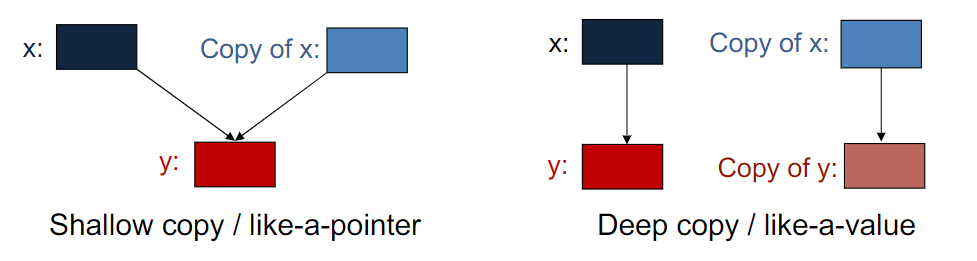
\includegraphics[width=14cm]{figures/shallow-and-deep.png}
    \caption{Shalow and deep copy}
    \label{fig:shallow-deep}
\end{figure}

Ordinarily, classes copy members of built-in types (other tha pointers) directly;
such members are values and hence ordinarily ought to behave like values. What we
do when we copy the pointer member determines whether the class has like-a-value or
like-a-pointer behavior.\\

For example, a like-a-pointer class:\\

\begin{lstlisting}[language=C++]
class StrLPVector{
    public:
    typedef std::vector<std::string>::size_type size_type;

    StrLPVector();
    StrLPVector(std::initializer_list<std::string> il);

    size_type size() const { return data->size(); }
    bool empty() const { return data->empty(); }

    // add and remove objects
    void push_back(const std::string &t) { data -> push_back(t); }
    void pop_back() { data-> pop_back(); }

    // element access
    std::string& front() { return data->front(); }
    std::string& back() { return data->back(); }

    private:
    std::shared_ptr<std::vector<std::string>> data;
    // write msg if data[i] isn't valid
};
\end{lstlisting}

For example, a like-a-value class:\\

\begin{lstlisting}[language=C++]
class StrLPVector {
    public:
    typedef std::vector<std::string>::size_type size_type;

    StrLPVector();
    StrLPVector(std::initializer_list<std::string> il);
    size_type size() const { return data.size(); }
    bool empty() const { return data.empty(); }

    // add and remove elements
    void push_back(const std::string &t) { data.push_back(t); }
    void pop_back() { data.pop_back(); };

    // element access
    std::string& front() { return data.front(); }
    std::string& back() { return data.back(); }

    private:
    std::vector<std::string> data;
    // write msg if data[i] isn't valid
};
\end{lstlisting}

\section{Implicit class-type conversions}

\texttt{C++} defines several automatic conversions among the built-in types. For example,
we can assign an \texttt{int} to a \texttt{double}, or pass an \texttt{int} to a function
that takes a \texttt{double} parameter.\\

Classes can define implicit conversion as well. Every constructor that can be called with a
single argument defines an implicit conversion to the class type. Such constructors are called
\textbf{converting constructors}. For example:\\

\begin{lstlisting}[language=C++]
class MatLabVector {
    vector<double> elem;

    public:
    MatLabVector(unsigned sz) : elem(sz, 0.) {}
    MatLabVector() = default;

    double& opeartor[](unsigned n);
    size_t size() const;

    MatLabVector operator+(const MatLabVector& other) const;
    MatLabVector operator*(double scalar) const;    
}
\end{lstlisting}

In this case, the \texttt{MatLabVector} constructor that takes an \texttt{unsigned} is a
defines implicit conversions from that type to a \texttt{MatLabVector}. We can use an 
\texttt{unsigned} wherever a \texttt{MatLabVector} is expected. For example:\\

\begin{lstlisting}[language=C++]
MatLabVector v1(10); // ok: direct initialization
v1 = 20; // ok: implicit conversion to MatLabVector

void f(MatLabVector);
f(10); // ok: implicit conversion to MatLabVector
\end{lstlisting}

This is very error prone (unless that is the desired behavior). To avoid this, we can use
the \texttt{explicit} keyword to prevent the compiler from using that constructor for implicit
conversions. For example:\\

\begin{lstlisting}[language=C++]
class MatLabVector {
    vector<double> elem;

    public:
    explicit MatLabVector(unsigned sz) : elem(sz, 0.) {}
    MatLabVector() = default;

    double& opeartor[](unsigned n);
    size_t size() const;

    MatLabVector operator+(const MatLabVector& other) const;
    MatLabVector operator*(double scalar) const;    
}

MatLabVector v1(10); // ok: direct initialization
v1 = 20; // error: no implicit conversion to MatLabVector

void f(MatLabVector);
f(10); // error: no implicit conversion to MatLabVector
\end{lstlisting}

Note that when we declare a constructor as \texttt{explicit}, we can only use that constructor
for direct initialization. We cannot use that constructor for copy initialization.\\

Although the compiler will not use an explicit constructor for an implicit conversion, we can
use such constructors explicitly to force a conversion. For example:\\

\begin{lstlisting}[language=C++]
MatLabVector v1(10); // ok: direct initialization
v1 = MatLabVector(20); // ok: explicit conversion to MatLabVector

v1 += 10; // error: no implicit conversion to MatLabVector
v1 += MatLabVector(10); // ok: explicit conversion to MatLabVector
\end{lstlisting}

\subsubsection{IMPORTANT:}

Consider the class \texttt{SalesData}, with its constructor \texttt{SalesData(const std::string)}.
Note that in this case, even if it is not explicit, only one implicit conversion is allowed.
For instance:\\

\begin{lstlisting}[language=C++]
// ERROR: requires two user-defined conversions:
// (1) convert "9-999-99999-9" to string
// (2) converst that (temporary) string to SalesData
item += "9-999-99999-9";

// OK: explicit conversion to string, implicit conversion to SalesData
item += string("9-999-99999-9");

// OK: implicit conversion to string, explicit conversion to SalesData
item += SalesData("9-999-99999-9");
\end{lstlisting}